%% Lee
%% In dissertation, change 
%    section* to chapter 
%    subsection* to section
%    subsubsection* to subsection

%\chapter{Preliminary Work}
\section{Preliminary Work}
\label{chap-five}

A small team within the NCSU ECE department, known as the DARPA Cortical team worked on accelerating two types of ANN known as Sparsey and HTM.
The work\cite{afrl_cortical} focused on comparing GPU implementations to one solution implemented using a pure ASIC and another solution using an ASIP.
Both Sparsey and HTM were implemented on a GPU and then power and speed were compared against the custom ASIC and ASIP solutions.
The DARPA Cortical team were able to demonstrate a overall performance improvement of better than two orders of magnitude over a GPU solution.
Although these designs employed only SRAM, and the size of the networks were constrained, the Cortical team demonstrated the 
potential for significant performance gains accelerating ANNs using ASIC or ASIP solutions.

This works research will propose a custom organized 3D-DRAM and special processing functions optimized for a family of popular ANNs. 
The solution is contained within a 3DIC footprint which inherently reduces power and increases bandwidth by keeping communication largely "on silicon".

To achieve the performance improvement over current generation GPU's, this work is targeting a 3DIC stack with ten's of thousands of
connections (TSV's) between die with logic running at approximately 1GHz.
The preliminary work carried out to date was a feasibility study to ensure the various research goals were achievable.
This work was based on a proposed partially re-organized version of the DRAM described in \cite{tezzaron:diram4}.
The initial re-organization proposes gaining access to an entire page within the DRAM. This will provide a raw DRAM bandwidth of
131Tbps spread over an array of 64 processing engines. 
The feasibility study involved:
\vspace{-2mm}
\begin{itemize}
  \itemsep-0.9mm
  \item a baseline application with eight CNNs \cite{krizhevsky2012imagenetPreso}
  \item a custom organized 3D-DRAM DiRAM4 \cite{tezzaron:diram4} 
  \item a power estimate of the primary energy consumers
  \item a real-estate study of the processing layer
\end{itemize}

During the DARPA Cortical project, a rudimentary design was completed that managed and performed floating point streaming operations.
The design included a streaming operation module, a circuit-switched Network-on-chip (NoC) module, a DMA engine, a memory controller and general control logic.
The synthesis results from that work were used in the feasibility study.
In addition, \cite{galal2011energy} was used to estimate fused multiply-accumulate (FMA) function power and size, \cite{liu2012compact} was used to estimate energy in TSV's in a die stack,
\cite{patti20142} was used to estimate real-estate for TSV's and \cite{tezzaron:diram4} was used to estimate energy associated with 3D-DRAM accesses.

For much of the feasibility study, this work used the Tezzaron DiRAM4 \cite{tezzaron:diram4}.
The area of the Tezzaron DiRAM4 die is approximately \SI{12.5}{\mm} by \SI{14.0}{\mm} or \SI{175}{\mm^2}.
This area was used as the baseline for the 3D stack die size.


For comparison, a typical GPU \cite{techpowerupteslak20c} has a silicon area of \SI{550}{\mm^2} using a \SI{28}{\nm} technology node 
and consumes in excess of \SI{100}{\W}.

Assuming these ANNs are processing images at a frame rate of 60fps, we will allocate \SI{10}{\ms} to complete computations
associated with the ANNs. We will also assume each NN is of a similar size to the CNN described in \cite{krizhevsky2012imagenetPreso}
which we estimate to have 2.1 billion floating point operations.
The floating point operations per second (FLOPS) estimate for eight NN's is therefore \SI{1.7}{TFLOPS} which correlates to a bandwidth of
\SI{54}{\tera bits/sec}.
The design target summary is shown in table \ref{tab:DesignTargets}.

% [h] forces that table to be here after the text above (not float)
\vspace{-5mm}
\begin{table}[h]
%  \captionsetup{justification=centering, skip=-5pt}
  \captionsetup{justification=centering, skip=3pt}
  \caption{Design targets}
  \label{tab:DesignTargets}
  \centering
%  \begin{center}
    % [lr] ~ left align col 0 and right align col 1
    % e.g. 4 columns could be lccr
    \begin{tabular}{lr}
      \toprule
      Parameter & Target \\
      \midrule
      Power     & \SI{40}{\W}   \\
      Bandwidth & \SI{54}{\tera\bit/\second} \\
      Die Area  & \SI{175}{\mm^2} \\
      \bottomrule
    \end{tabular}
%  \end{center}
\end{table}
\vspace{-5mm}
In the feasibility study, we assume the DiRAM4 port can be re-organized to provide access to the \SI{4096}{\bit} cacheline. 
The DRAM page open and close constraints are such that we can only gain access to a page every two clocks. Therefore, the port manager
transfers 2048 bits down the stack bus every clock period of \SI{1}{\ns}.

With 64-ports this provides a raw bandwidth of \SI{131}{\tera bits/sec}. This work anticipates that the data structure resulting from the research will result in 
the solution being able to meet or exceed the 42\% bandwidth utilization of the baseline.

The port manager shown in \fref{fig:blockDiagram} will transmit computation operands to a processing element (PE) on the processing layer.
The PE will contain a number of executions lanes and each execution lane can receive up to two operands every clock
cycle from the port manager. A "float" is 32 bits, therefore the stack bus width of 2048 bits will support 32 execution lanes on the corresponding PE.
The DiRAM4 has 64-ports, therefore the processing layer will support 64 PE's with each PE supporting 32 execution lanes.
In practice, each execution lane will be performing a multiply-accumulate on the weight/input tuple from the stack bus.
Therefore, for the PE design we assume 32 FMA's, a small amount of SRAM, a 32-lane NCSU SIMD core
and dma/control logic whose size is estimated from \cite{afrl_cortical}.

%\subsection*{Power Dissipation}
The overall power estimate is based on estimates of the PE FMA's, the SIMD, the DRAM, the TSV interconnects and an estimate for the
general control logic.
The main concern with respect to area is supporting the number of computational units in each PE within the processing layer. 
The area of each PE is based on the SIMD, FMA, SRAM, DMA and control logic.

The SIMD and control logic is based on the work from \cite{afrl_cortical}. The area and power of the FMA is based on \cite{galal2011energy}.
The DRAM power is based on \cite{tezzaron:diram4}.
The overall power estimate is shown in Table \ref{tab:powerEstimates}.
%\subsection*{Area}
The available area is based on the size of the DiRAM4. The area of the PE is estimated by scaling the area of the individual units.
The area was estimated using nations of best through worst case scaling numbers from \cite{schabel2014energy}
The PE area for the various scaling can be seen in \fref{fig:peAreaWithScaling}. Only the estimated area using worst case scaling exceeds the area available.

\begin{figure}[h]
\centering
\captionsetup{justification=centering}
    \begin{subtable}{.50\textwidth}
    %  \captionsetup{justification=centering, skip=-5pt}
      \centering
    %  \begin{center}
        % [lr] ~ left align col 0 and right align col 1
        % e.g. 4 columns could be lccr
        \resizebox{\textwidth}{!}{ % Scale table
        \begin{tabular}{r|ccc}
          \toprule
                         & \multicolumn{3}{c}{Technology} \\
                    Unit & \SI{130}{\nm} & \SI{65}{\nm} & \SI{45}{\nm}  \\
          \hline
          SIMD (32-lane) & 3200000 \\
                    DMA  &               & 368000  \\
      Memory Controller  &               & 294000  \\
                Control  &               & 1032000 \\
                   SRAM  &               & 740098  \\
                    FMA  &               &              & 405440 \\
          \bottomrule
        \end{tabular}
        }
      \captionsetup{justification=centering, skip=9pt}
      \vspace{-1mm}
      \caption{Original area estimates}
      \label{tab:areaEstimates}
    %  \end{center}
    \end{subtable}
    \hfill
    %\vfill
    \begin{subtable}{.45\textwidth}
    %  \captionsetup{justification=centering, skip=-5pt}
      \centering
    %  \begin{center}
        % [lr] ~ left align col 0 and right align col 1
        % e.g. 4 columns could be lccr
        \resizebox{\textwidth}{!}{%
        \begin{tabular}{r|cccc}
          \toprule
                         & \multicolumn{4}{c}{Technology} \\
                 Source  & \SI{130}{\nm} & \SI{65}{\nm} & \SI{45}{\nm} & \SI{32}{\nm}  \\  \cline{1-1}
          \hline  % instead of \midrule %midrule doesnt overlap with column lines
                    ITRS & 8.00          & 2.00         & 1.00         & 0.66\\ %\cline{2-2}
                    PTM  & 8.00          & 2.00         & 1.00         & 0.50\\
                  Intel  & 2.37          & 1.33         & 1.00         & 0.75\\
          \bottomrule
        \end{tabular}
        }
      \captionsetup{justification=centering, skip=9pt}
      \vspace{3mm}
      \caption{Scaling numbers (from \cite{schabel2014energy})}
      \label{tab:scalingNumbers}
    %  \end{center}
    \end{subtable}
\vspace{-2mm}
\caption{Original area estimates and scaling numbers}
\label{fig:areaAndScalingEstimates}
\end{figure}

%The estimated power dissipation of \SI{40}{\W} and supporting eight baseline ANNs suggests an overall improvement over a GPU solution of 20x.
\vspace{-1cm}
\begin{figure}[h]
\centering
\captionsetup{justification=centering}
    \begin{subtable}{.3\textwidth}
    %  \captionsetup{justification=centering, skip=-5pt}
      \centering
    %  \begin{center}
        % [lr] ~ left align col 0 and right align col 1
        % e.g. 4 columns could be lccr
        \begin{tabular}{ccc}
          \toprule
          Function & Power \\
          \midrule
          FMA      & \SI{4.7}{\W}  \\
          General  & \SI{16}{\W}   \\
          SIMD     & \SI{1.6}{\W}  \\
          DRAM     & \SI{3.4}{\W}  \\
          TSV's    & \SI{13.2}{\W} \\
          \midrule                 
          Total    & \SI{38.9}{\W} \\
          \bottomrule
        \end{tabular}
      \captionsetup{justification=centering, skip=9pt}
      \vspace{0.5cm}
      \caption{Power estimates}
      \label{tab:powerEstimates}
    %  \end{center}
    \end{subtable}
    \begin{subfigure}{.65\textwidth}
      \centering
      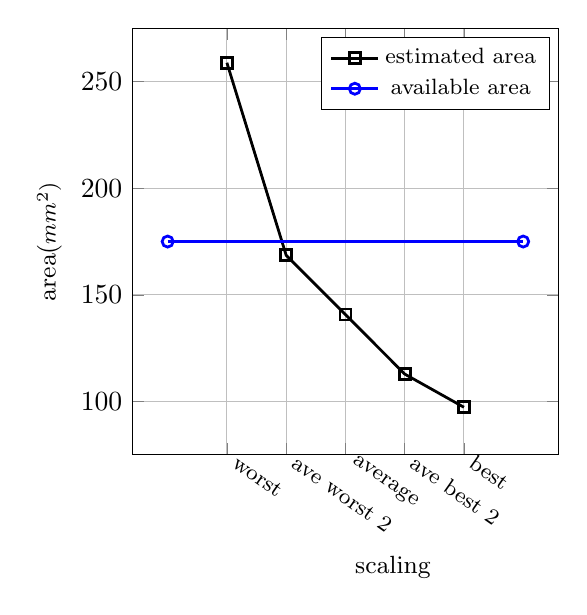
\begin{tikzpicture}
          \begin{axis}[
              height=7cm,
              width=7cm,
              grid=major,
              ylabel={\small area(\footnotesize $mm^2$)},
              %ylabel style={rotate=90,left},
              ylabel near ticks,
              ymin=75,ymax=275,
              symbolic x coords={left, worst, ave worst 2, average, ave best 2, best, right},
              xtick=data,
              xticklabels={\footnotesize worst, \footnotesize ave worst 2, \footnotesize average, \footnotesize ave best 2, \footnotesize best },
              x tick label style={rotate=325,anchor=west},
              xlabel={\small scaling},
              xlabel style={below right},
              %nodes near coords,
              %nodes near coords align={vertical},
          ]
          \addplot[color=black,mark=square,line width=1pt,-] coordinates {
                 (worst,           258.82  )
                 (ave worst 2,     168.57  )
                 (average,         140.81  )
                 (ave best 2,      112.89  )
                 (best,             97.32  )
              };
          \addlegendentry{\footnotesize estimated area}
          \addplot[color=blue,mark=o,line width=1pt,-] coordinates {
                 (left,          175  )
                 (right,         175  )
          };
          \addlegendentry{\footnotesize available area}
          \end{axis}
      \end{tikzpicture}
      \captionsetup{justification=centering, skip=3pt}
      \caption{PE layer area estimate after scaling (using \cite{schabel2014energy})}
      \label{fig:peAreaWithScaling}
    \end{subfigure}%
\caption{Power and area estimates}
\label{fig:powerAndAreaEstimates}
\end{figure}

    
